\section{Methods}
\label{sec:methods}

\subsection{Dataset}

We use the Depresjon dataset released by Simula Research Laboratory \cite{garcia2018depresjon}, which contains continuous wrist actigraphy recordings from 55 participants: 32 healthy controls and 23 individuals with diagnosed mood disorders. All recordings were collected using an Actiwatch device (Cambridge Neurotechnology Ltd., model AW4) worn on the right wrist and sampled at 32\,Hz using a piezoelectric accelerometer, with activity counts pre-aggregated to one-minute epochs. The dataset includes demographic metadata and Montgomery-\r{A}sberg Depression Rating Scale (MADRS) scores for the condition group. Among the 23 condition participants, 8 carry a diagnosis of bipolar disorder (Bipolar I or Bipolar II) and 15 carry a diagnosis of Unipolar Depressive Disorder. This 8:15 split is the primary class imbalance challenge for our differential diagnosis task. Table~\ref{tab:dataset} summarizes the key demographic and recording characteristics of both groups.

\begin{table}
\centering
\caption{Depresjon dataset participant characteristics.}
\label{tab:dataset}
\begin{tabular}{lcc}
\toprule
\textbf{Characteristic} & \textbf{Controls (n=32)} & \textbf{Condition (n=23)} \\
\midrule
Sex (F/M) & 20 / 12 & 10 / 13 \\
Mean age (years) & $38.2 \pm 13.0$ & $42.8 \pm 11.0$ \\
Recording length (days) & $12.6 \pm 3.3$ & $12.7 \pm 2.8$ \\
Range of recordings & 8--20 days & 5--18 days \\
Mean MADRS score & N/A & $22.7 \pm 4.8$ \\
Diagnosis split & N/A & 15 Unipolar / 8 Bipolar \\
\bottomrule
\end{tabular}
\end{table}

\begin{figure}
\centering
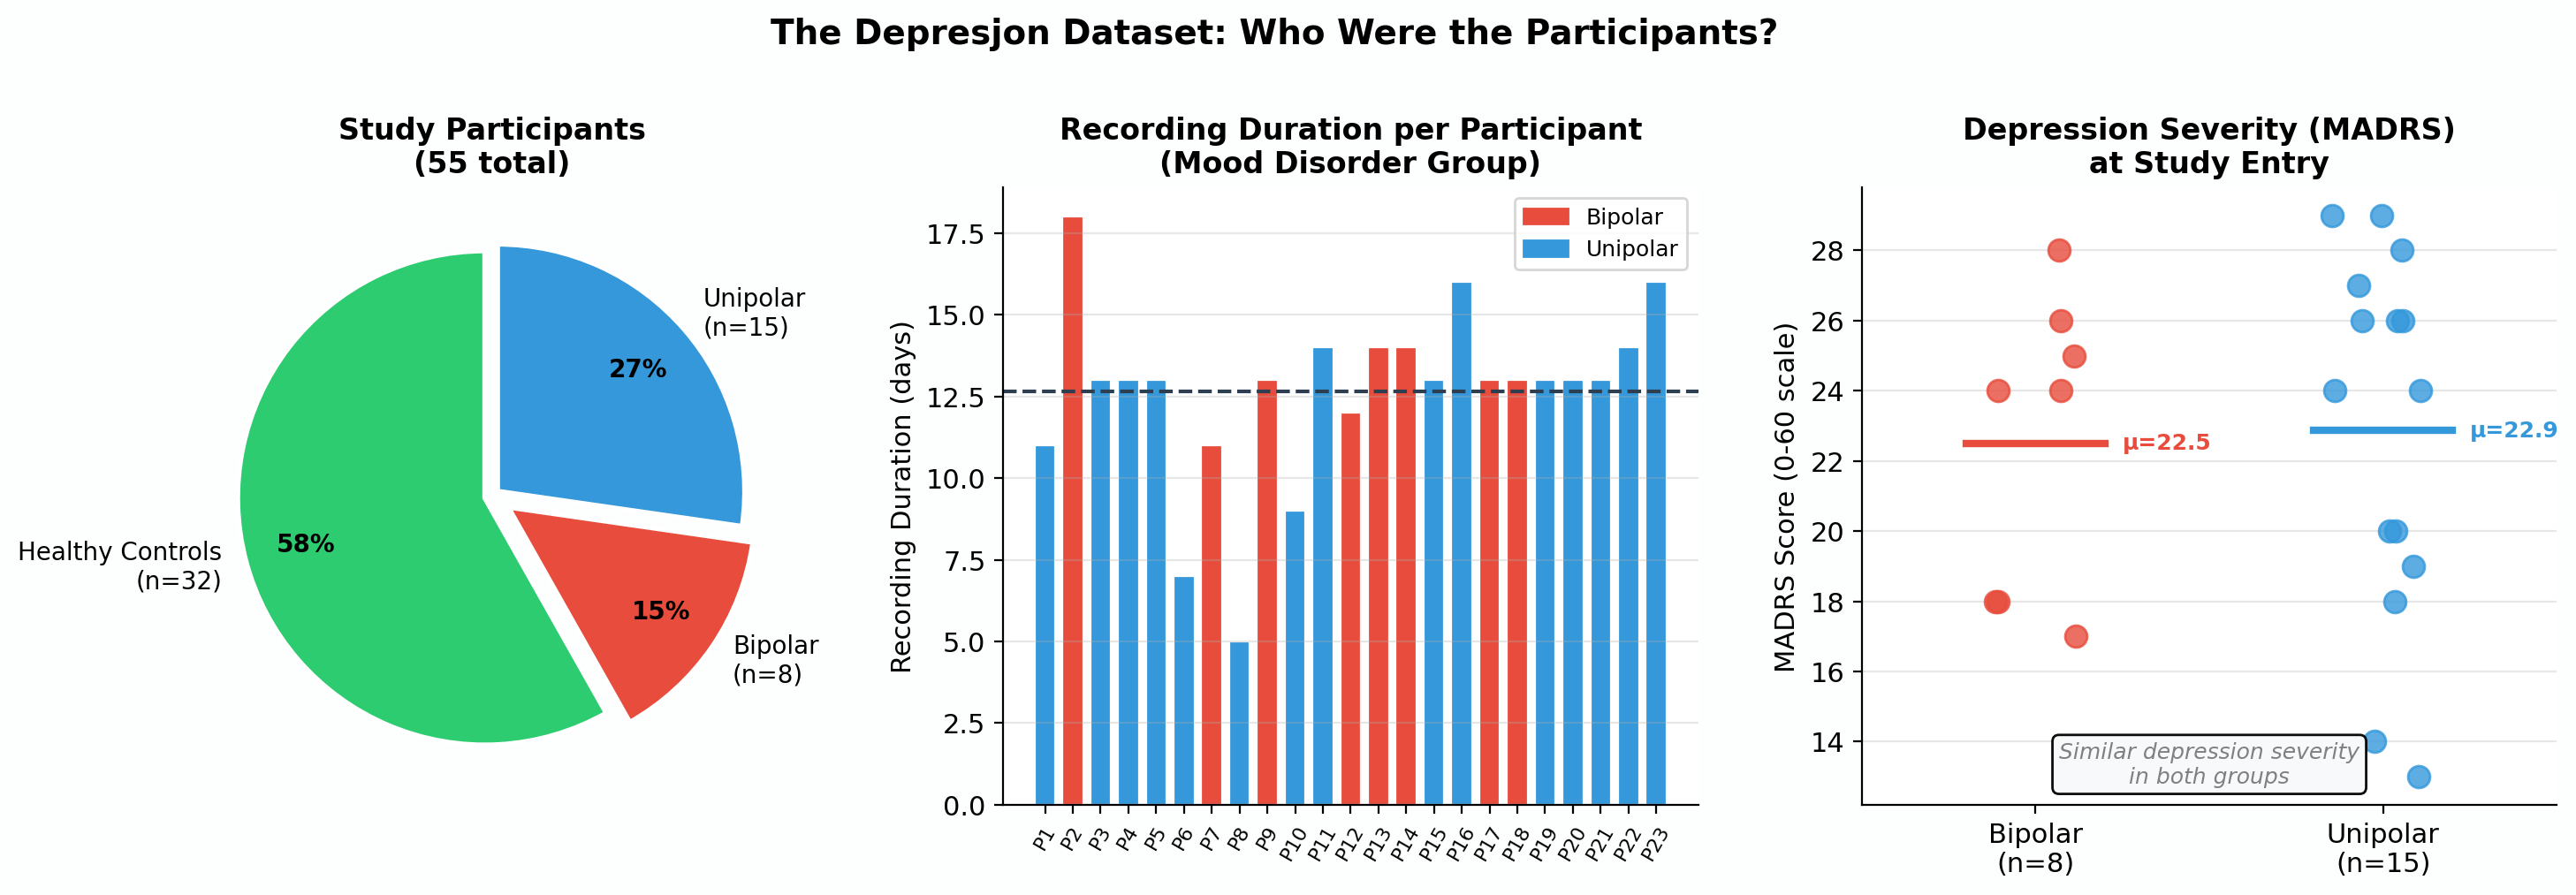
\includegraphics[width=\linewidth]{images/figA_dataset_overview.png}
\caption{Depresjon dataset overview. \textit{Left:} Participant composition (32 healthy controls, 8 bipolar, 15 unipolar). \textit{Centre:} Recording duration per condition participant. \textit{Right:} MADRS depression severity scores for bipolar vs.\ unipolar groups (means nearly identical: 22.5 vs.\ 22.9).}
\label{fig:dataset_overview}
\end{figure}

\begin{figure}
\centering
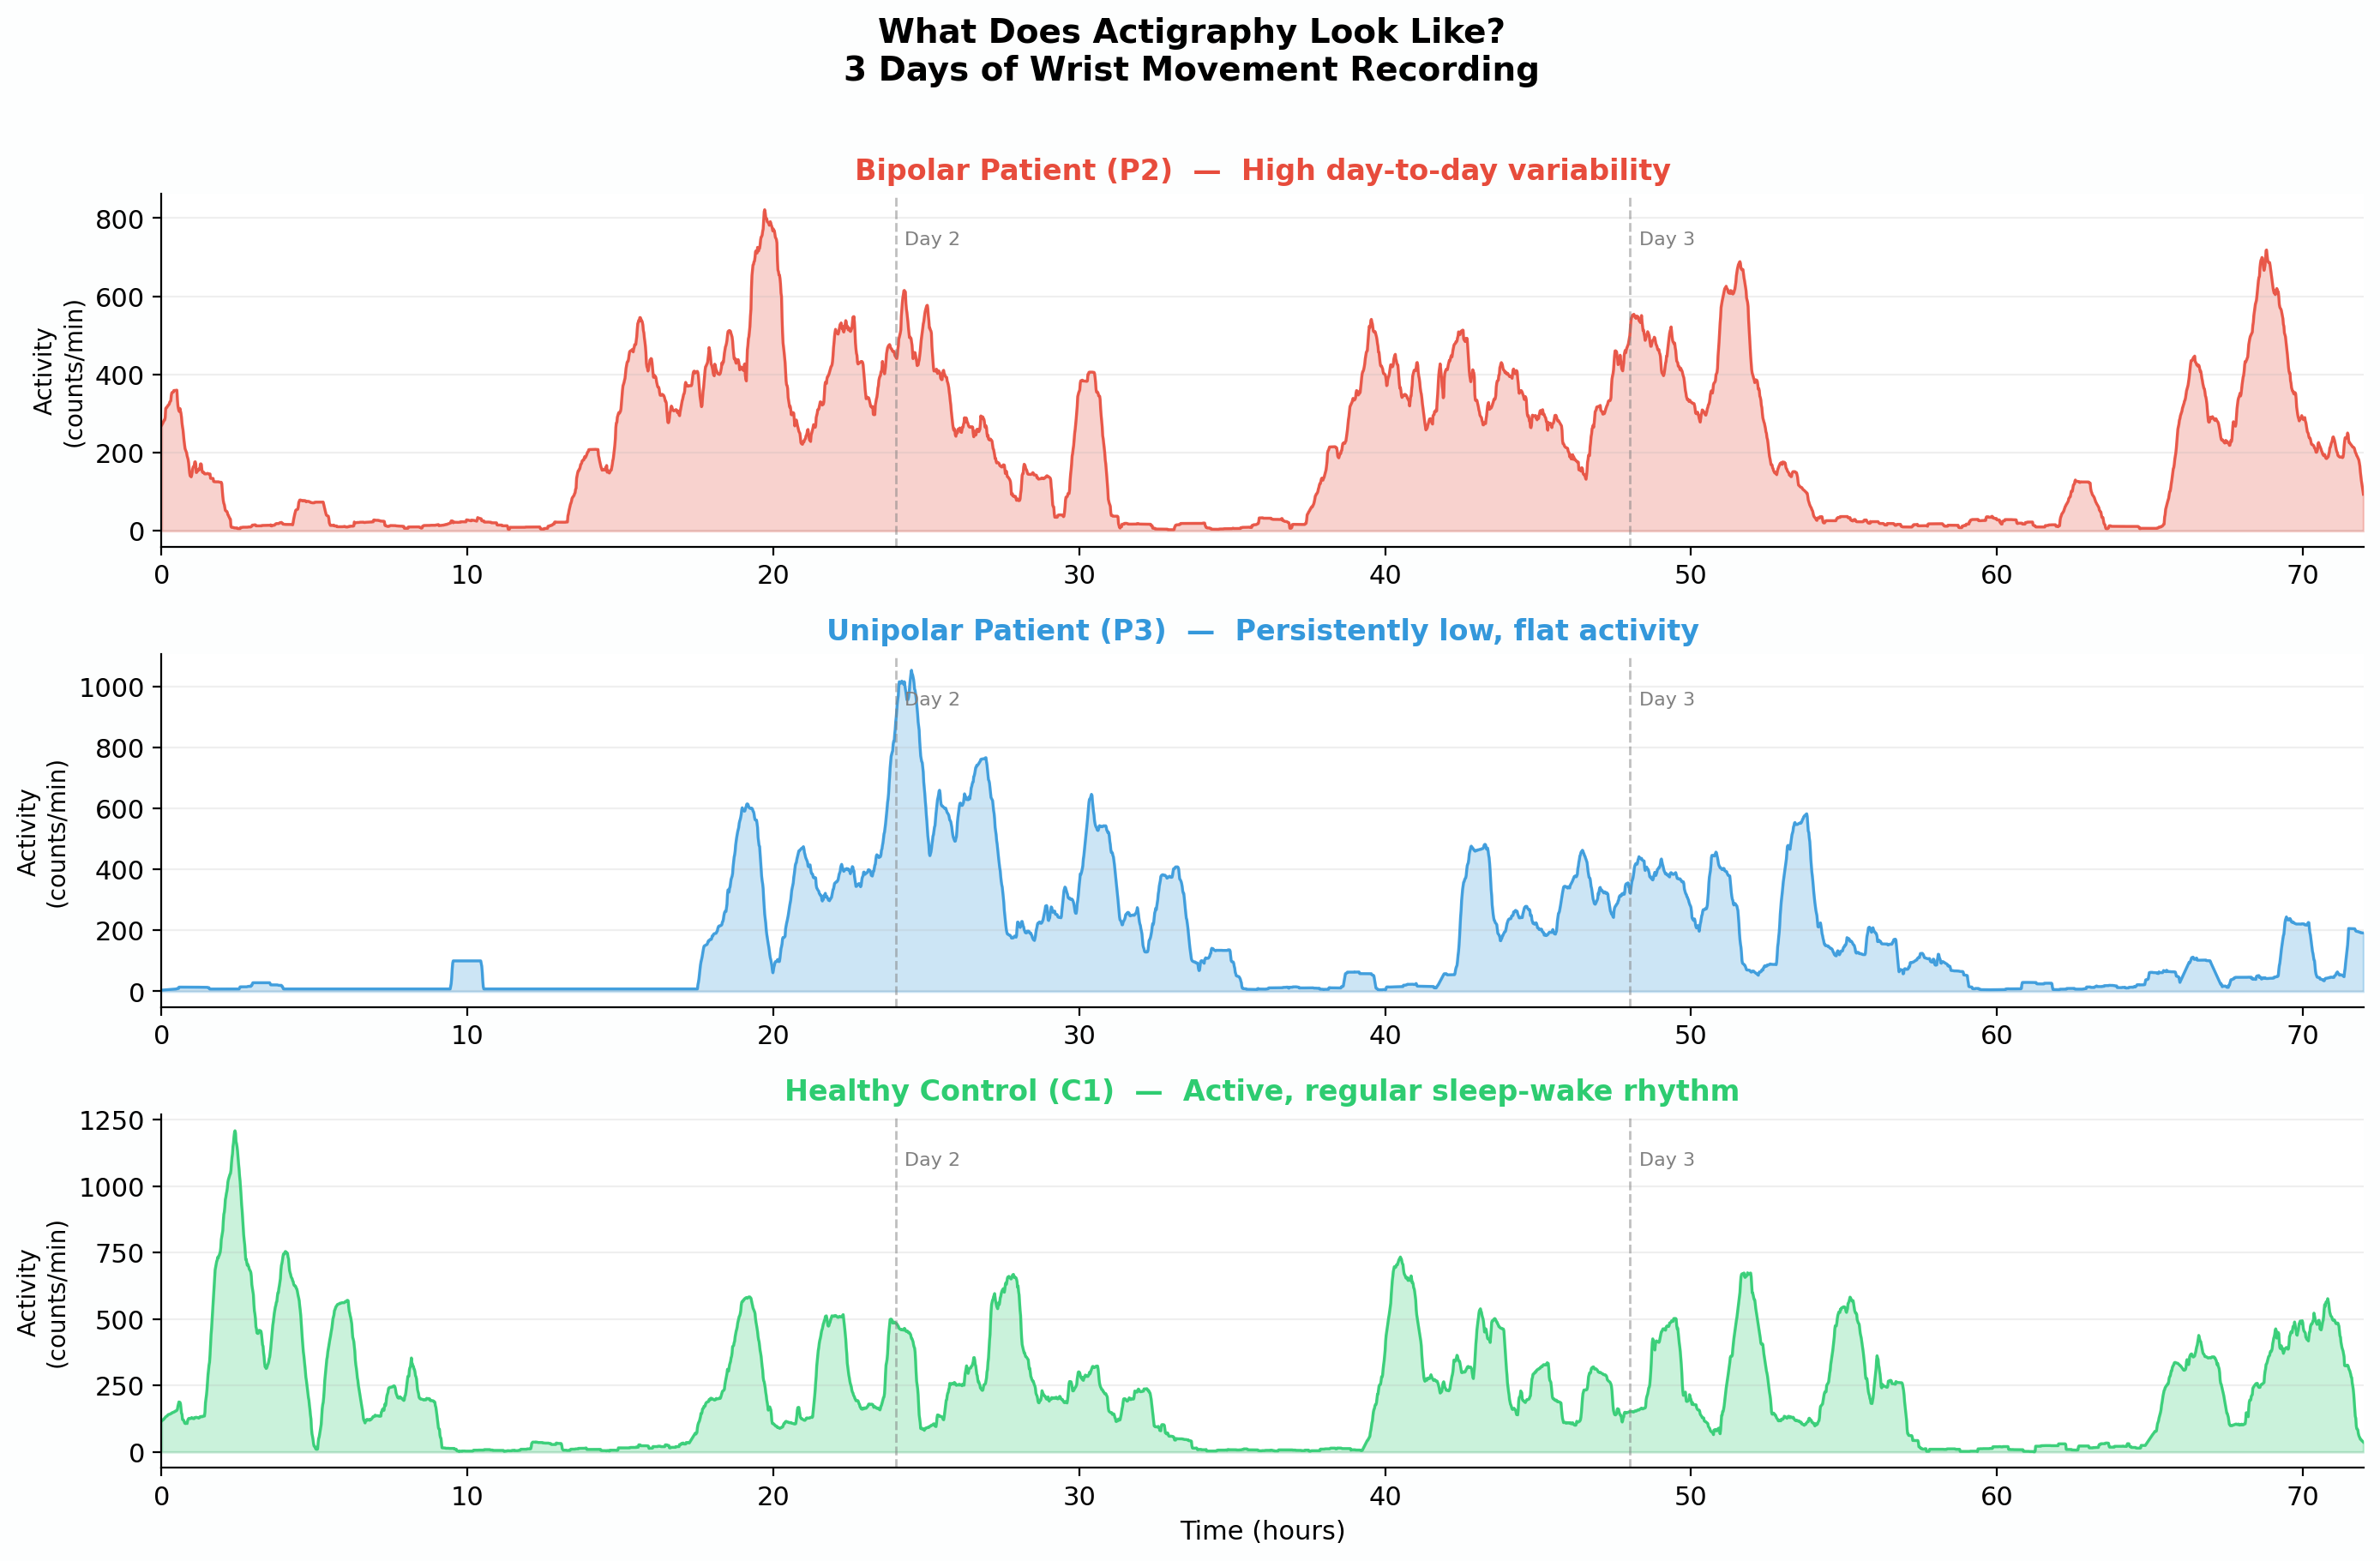
\includegraphics[width=\linewidth]{images/figB_sample_actigraphy.png}
\caption{Three days of raw wrist actigraphy for representative participants. Bipolar patient (P2) shows high day-to-day variability; unipolar patient (P3) shows persistently low, flat activity; healthy control (C1) shows a regular, active sleep-wake rhythm.}
\label{fig:sample_actigraphy}
\end{figure}

\subsection{Preprocessing}

Each participant's raw activity count time series is independently normalized to zero mean and unit variance using z-score standardization. Normalization is computed per participant to remove inter-subject baseline differences in overall activity level that are unrelated to diagnosis. Following normalization, each recording is segmented into non-overlapping 1,440-minute (24-hour) windows, with a 60-minute stride applied during training to increase the number of available training examples. Each window inherits the diagnostic label of the participant from whom it was drawn. Participant-level stratified splits (80\% train, 10\% validation, 10\% test) are applied before windowing, ensuring that no participant's data appears in more than one split and preventing data leakage between train and test. To give a sense of scale, a typical participant with a 12-day recording contributes approximately 12 non-overlapping 24-hour windows; with the 60-minute stride applied during training this count rises further, which is why 44 training participants collectively yield over 20,000 training windows despite the small participant count. All diagnostic labels are assigned at the participant level before windowing, so every window generated from a given participant carries that participant's diagnosis.

\subsection{Model Architecture}

We design a hybrid 1D-CNN-LSTM architecture motivated by the dual-scale temporal structure of actigraphy data: short-term kinetic texture (minute-to-minute activity bursts, rest-onset transitions) and long-range circadian patterns (day-to-day rhythmic drift, sleep-wake cycle variability). The CNN component handles local pattern extraction, and the LSTM component handles multi-day information integration.

\subsubsection{Local Feature Extraction (1D-CNN).}
Two sequential convolutional blocks are applied to the raw activity sequence. Each block consists of a 1D convolutional layer followed by batch normalization \cite{ioffe2015batchnorm}, ReLU activation, and max pooling with stride 2. The first block uses 64 filters with kernel size 7, and the second uses 128 filters with kernel size 5. The output is a sequence of higher-level feature vectors summarizing local movement texture at progressively coarser time scales.

\subsubsection{Long-Range Dependency Tracking (LSTM).}
The CNN output feature maps are passed as a sequence into a single-layer LSTM \cite{hochreiter1997lstm} with 128 hidden units. The LSTM's gated memory mechanism allows it to selectively retain information from earlier time steps, enabling it to track multi-day patterns across the full recording period.

\subsubsection{Classification Head.}
The final LSTM hidden state passes through two fully connected layers with 256 and 64 units respectively, each followed by ReLU activation and Dropout \cite{srivastava2014dropout} with probability 0.4. The output layer applies softmax over the target classes. Table~\ref{tab:architecture} provides a complete layer-by-layer description.

\begin{table}
\centering
\caption{1D-CNN-LSTM architecture. Input is a $T \times 1$ raw activity sequence.}
\label{tab:architecture}
\begin{tabular}{llll}
\toprule
\textbf{Stage} & \textbf{Layer} & \textbf{Config} & \textbf{Output} \\
\midrule
\multirow{2}{*}{CNN Block 1} & Conv1D & 64 filters, k=7 & $T \times 64$ \\
 & MaxPool1D & stride=2 & $T/2 \times 64$ \\
\midrule
\multirow{2}{*}{CNN Block 2} & Conv1D & 128 filters, k=5 & $T/2 \times 128$ \\
 & MaxPool1D & stride=2 & $T/4 \times 128$ \\
\midrule
Recurrent & LSTM & 128 hidden units & 128 \\
\midrule
\multirow{2}{*}{FC Head} & Linear + ReLU + Drop(0.4) & 256 units & 256 \\
 & Linear + ReLU + Drop(0.4) & 64 units & 64 \\
\midrule
Output & Linear + Softmax & $C$ classes & $C$ \\
\bottomrule
\end{tabular}
\end{table}

The total parameter count for the baseline architecture is 223,682, trained end-to-end from random initialization using the Adam optimizer \cite{kingma2015adam} with learning rate $10^{-3}$ and weight decay $10^{-4}$. Training runs for a maximum of 50 epochs with early stopping at patience 10 on validation loss. The primary evaluation metric for the healthy-versus-depressed task is macro-averaged F1-Score. For all bipolar-versus-unipolar experiments, the primary metric is ROC-AUC \cite{fawcett2006roc}, which is robust to class imbalance and evaluates the model's ability to rank positive instances above negative instances across all decision thresholds.

\begin{figure}
\centering
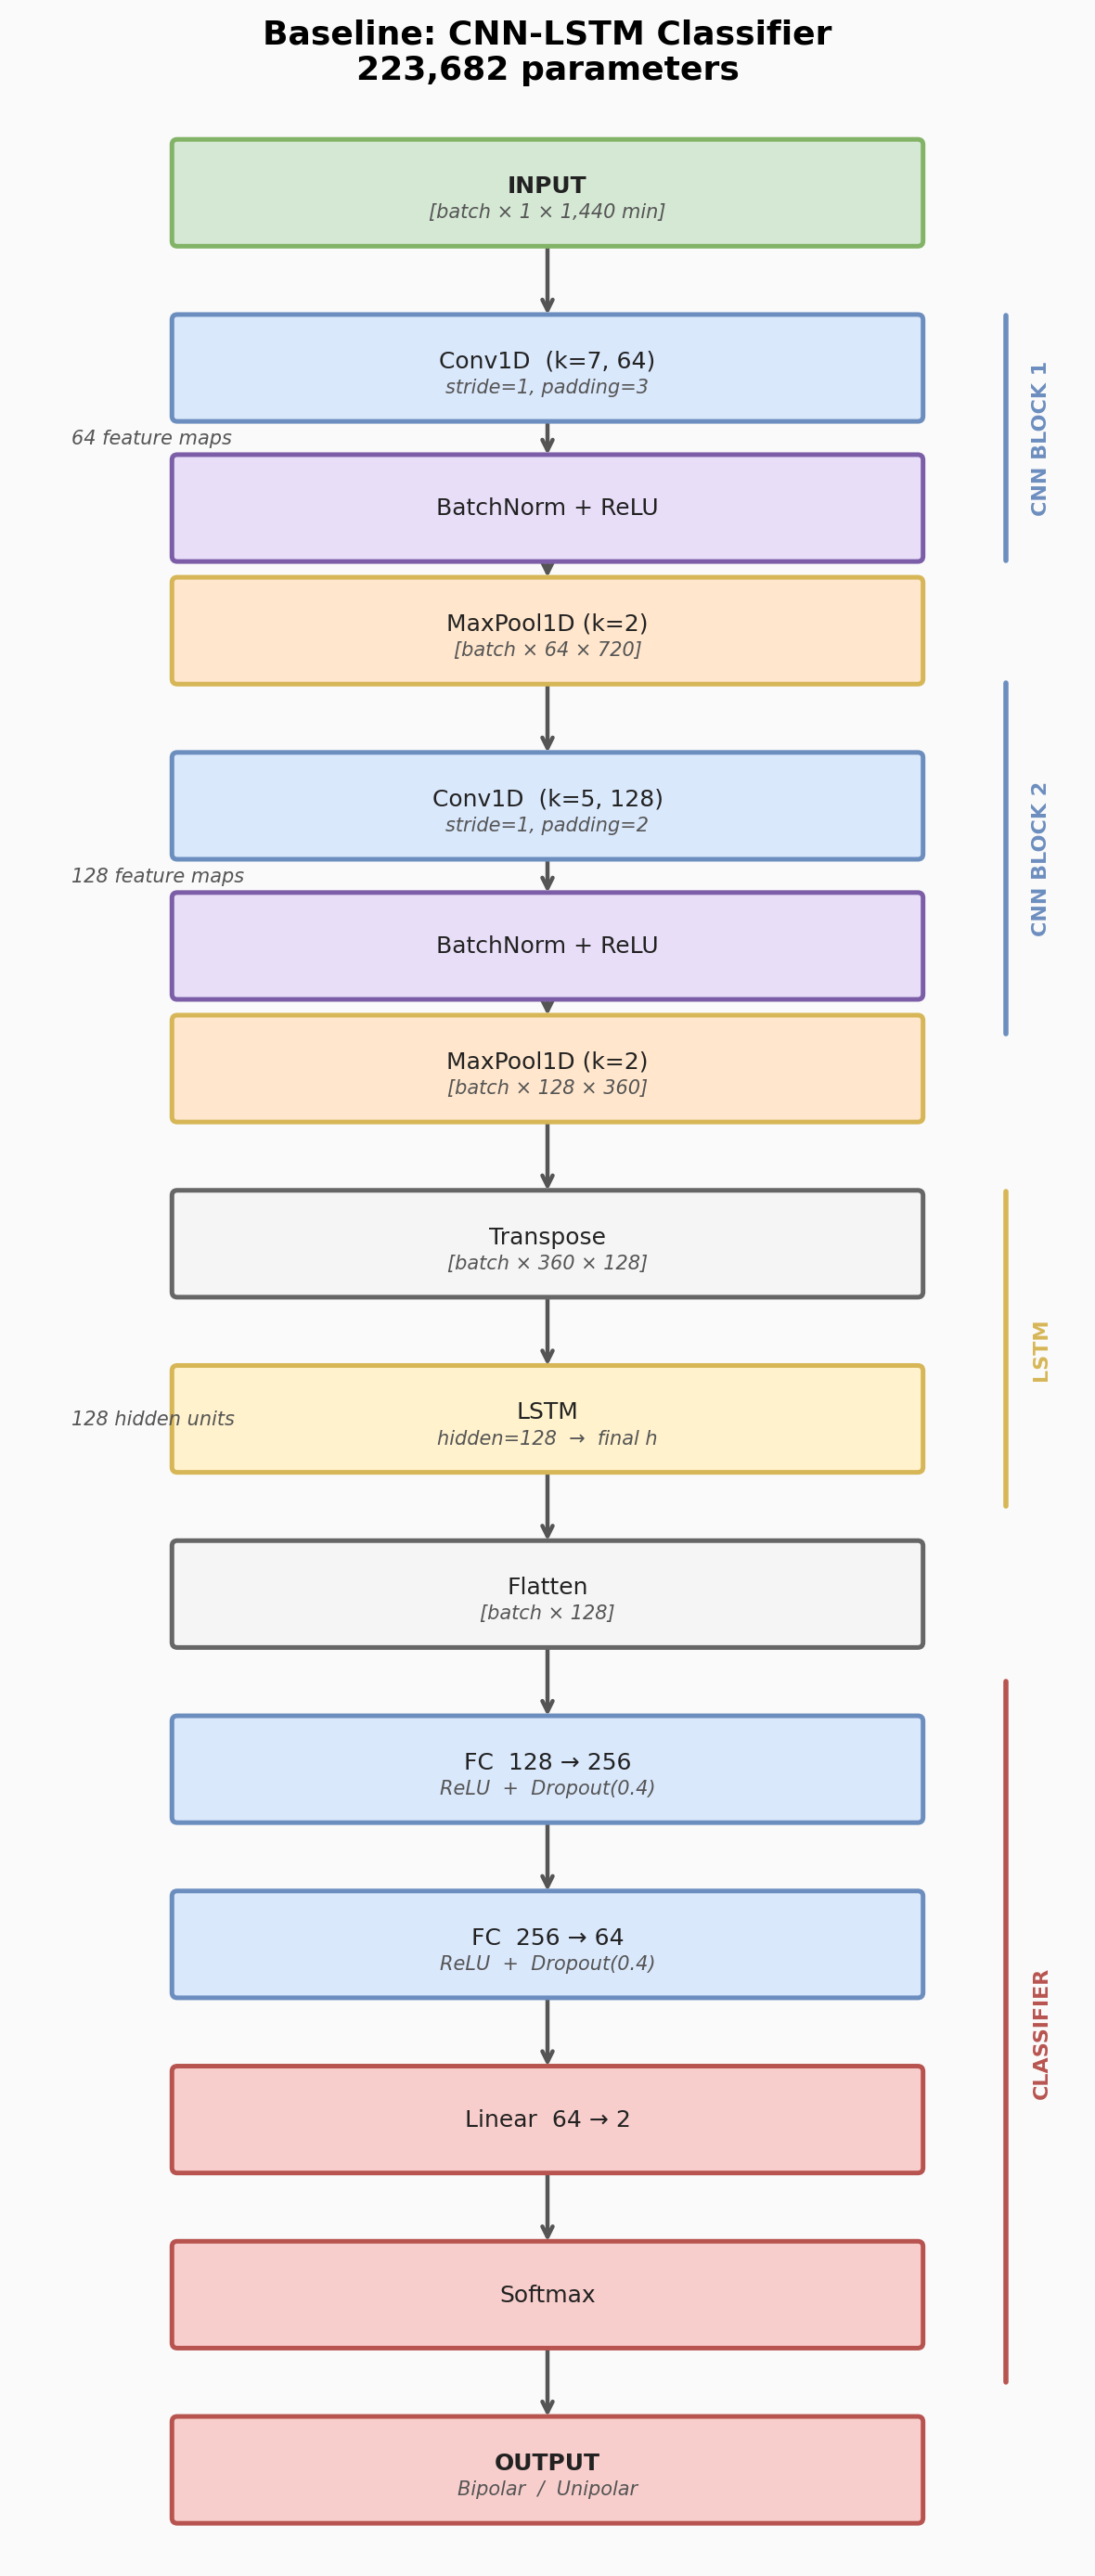
\includegraphics[width=0.55\linewidth]{images/figJ_arch_baseline_cnnlstm.png}
\caption{Baseline 1D-CNN-LSTM architecture (223,682 parameters). Two CNN blocks extract local kinetic features; a single LSTM layer integrates multi-day temporal context; two FC layers produce the final classification.}
\label{fig:arch_baseline}
\end{figure}
